\documentclass[1p]{elsarticle_modified}
%\bibliographystyle{elsarticle-num}

%\usepackage[colorlinks]{hyperref}
%\usepackage{abbrmath_seonhwa} %\Abb, \Ascr, \Acal ,\Abf, \Afrak
\usepackage{amsfonts}
\usepackage{amssymb}
\usepackage{amsmath}
\usepackage{amsthm}
\usepackage{scalefnt}
\usepackage{amsbsy}
\usepackage{kotex}
\usepackage{caption}
\usepackage{subfig}
\usepackage{color}
\usepackage{graphicx}
\usepackage{xcolor} %% white, black, red, green, blue, cyan, magenta, yellow
\usepackage{float}
\usepackage{setspace}
\usepackage{hyperref}

\usepackage{tikz}
\usetikzlibrary{arrows}

\usepackage{multirow}
\usepackage{array} % fixed length table
\usepackage{hhline}

%%%%%%%%%%%%%%%%%%%%%
\makeatletter
\renewcommand*\env@matrix[1][\arraystretch]{%
	\edef\arraystretch{#1}%
	\hskip -\arraycolsep
	\let\@ifnextchar\new@ifnextchar
	\array{*\c@MaxMatrixCols c}}
\makeatother %https://tex.stackexchange.com/questions/14071/how-can-i-increase-the-line-spacing-in-a-matrix
%%%%%%%%%%%%%%%

\usepackage[normalem]{ulem}

\newcommand{\msout}[1]{\ifmmode\text{\sout{\ensuremath{#1}}}\else\sout{#1}\fi}
%SOURCE: \msout is \stkout macro in https://tex.stackexchange.com/questions/20609/strikeout-in-math-mode

\newcommand{\cancel}[1]{
	\ifmmode
	{\color{red}\msout{#1}}
	\else
	{\color{red}\sout{#1}}
	\fi
}

\newcommand{\add}[1]{
	{\color{blue}\uwave{#1}}
}

\newcommand{\replace}[2]{
	\ifmmode
	{\color{red}\msout{#1}}{\color{blue}\uwave{#2}}
	\else
	{\color{red}\sout{#1}}{\color{blue}\uwave{#2}}
	\fi
}

\newcommand{\Sol}{\mathcal{S}} %segment
\newcommand{\D}{D} %diagram
\newcommand{\A}{\mathcal{A}} %arc


%%%%%%%%%%%%%%%%%%%%%%%%%%%%%5 test

\def\sl{\operatorname{\textup{SL}}(2,\Cbb)}
\def\psl{\operatorname{\textup{PSL}}(2,\Cbb)}
\def\quan{\mkern 1mu \triangleright \mkern 1mu}

\theoremstyle{definition}
\newtheorem{thm}{Theorem}[section]
\newtheorem{prop}[thm]{Proposition}
\newtheorem{lem}[thm]{Lemma}
\newtheorem{ques}[thm]{Question}
\newtheorem{cor}[thm]{Corollary}
\newtheorem{defn}[thm]{Definition}
\newtheorem{exam}[thm]{Example}
\newtheorem{rmk}[thm]{Remark}
\newtheorem{alg}[thm]{Algorithm}

\newcommand{\I}{\sqrt{-1}}
\begin{document}

%\begin{frontmatter}
%
%\title{Boundary parabolic representations of knots up to 8 crossings}
%
%%% Group authors per affiliation:
%\author{Yunhi Cho} 
%\address{Department of Mathematics, University of Seoul, Seoul, Korea}
%\ead{yhcho@uos.ac.kr}
%
%
%\author{Seonhwa Kim} %\fnref{s_kim}}
%\address{Center for Geometry and Physics, Institute for Basic Science, Pohang, 37673, Korea}
%\ead{ryeona17@ibs.re.kr}
%
%\author{Hyuk Kim}
%\address{Department of Mathematical Sciences, Seoul National University, Seoul 08826, Korea}
%\ead{hyukkim@snu.ac.kr}
%
%\author{Seokbeom Yoon}
%\address{Department of Mathematical Sciences, Seoul National University, Seoul, 08826,  Korea}
%\ead{sbyoon15@snu.ac.kr}
%
%\begin{abstract}
%We find all boundary parabolic representation of knots up to 8 crossings.
%
%\end{abstract}
%\begin{keyword}
%    \MSC[2010] 57M25 
%\end{keyword}
%
%\end{frontmatter}

%\linenumbers
%\tableofcontents
%
\newcommand\colored[1]{\textcolor{white}{\rule[-0.35ex]{0.8em}{1.4ex}}\kern-0.8em\color{red} #1}%
%\newcommand\colored[1]{\textcolor{white}{ #1}\kern-2.17ex	\textcolor{white}{ #1}\kern-1.81ex	\textcolor{white}{ #1}\kern-2.15ex\color{red}#1	}

{\Large $\underline{12n_{0869}~(K12n_{0869})}$}

\setlength{\tabcolsep}{10pt}
\renewcommand{\arraystretch}{1.6}
\vspace{1cm}\begin{tabular}{m{100pt}>{\centering\arraybackslash}m{274pt}}
\multirow{5}{120pt}{
	\centering
	\includegraphics[width=112pt]{../../../GIT/diagram.site/Diagrams/png/2958_12n_0869.png}\\
\ \ \ A knot diagram\footnotemark}&
\allowdisplaybreaks
\textbf{Linearized knot diagam} \\
\cline{2-2}
 &
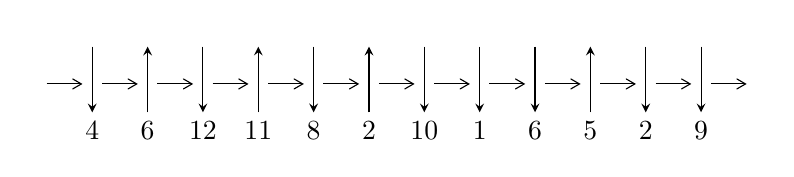
\begin{tikzpicture}[x=20pt, y=17pt]
	% nodes
	\node (C0) at (0, 0) {};
	\node (C1) at (1, 0) {};
	\node (C1U) at (1, +1) {};
	\node (C1D) at (1, -1) {4};

	\node (C2) at (2, 0) {};
	\node (C2U) at (2, +1) {};
	\node (C2D) at (2, -1) {6};

	\node (C3) at (3, 0) {};
	\node (C3U) at (3, +1) {};
	\node (C3D) at (3, -1) {12};

	\node (C4) at (4, 0) {};
	\node (C4U) at (4, +1) {};
	\node (C4D) at (4, -1) {11};

	\node (C5) at (5, 0) {};
	\node (C5U) at (5, +1) {};
	\node (C5D) at (5, -1) {8};

	\node (C6) at (6, 0) {};
	\node (C6U) at (6, +1) {};
	\node (C6D) at (6, -1) {2};

	\node (C7) at (7, 0) {};
	\node (C7U) at (7, +1) {};
	\node (C7D) at (7, -1) {10};

	\node (C8) at (8, 0) {};
	\node (C8U) at (8, +1) {};
	\node (C8D) at (8, -1) {1};

	\node (C9) at (9, 0) {};
	\node (C9U) at (9, +1) {};
	\node (C9D) at (9, -1) {6};

	\node (C10) at (10, 0) {};
	\node (C10U) at (10, +1) {};
	\node (C10D) at (10, -1) {5};

	\node (C11) at (11, 0) {};
	\node (C11U) at (11, +1) {};
	\node (C11D) at (11, -1) {2};

	\node (C12) at (12, 0) {};
	\node (C12U) at (12, +1) {};
	\node (C12D) at (12, -1) {9};
	\node (C13) at (13, 0) {};

	% arrows
	\draw[->,>={angle 60}]
	(C0) edge (C1) (C1) edge (C2) (C2) edge (C3) (C3) edge (C4) (C4) edge (C5) (C5) edge (C6) (C6) edge (C7) (C7) edge (C8) (C8) edge (C9) (C9) edge (C10) (C10) edge (C11) (C11) edge (C12) (C12) edge (C13) ;	\draw[->,>=stealth]
	(C1U) edge (C1D) (C2D) edge (C2U) (C3U) edge (C3D) (C4D) edge (C4U) (C5U) edge (C5D) (C6D) edge (C6U) (C7U) edge (C7D) (C8U) edge (C8D) (C9U) edge (C9D) (C10D) edge (C10U) (C11U) edge (C11D) (C12U) edge (C12D) ;
	\end{tikzpicture} \\
\hhline{~~} \\& 
\textbf{Solving Sequence} \\ \cline{2-2} 
 &
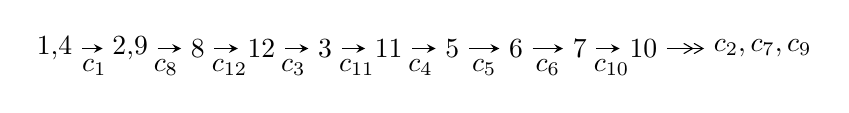
\begin{tikzpicture}[x=23pt, y=7pt]
	% node
	\node (A0) at (-1/8, 0) {1,4};
	\node (A1) at (17/16, 0) {2,9};
	\node (A2) at (17/8, 0) {8};
	\node (A3) at (25/8, 0) {12};
	\node (A4) at (33/8, 0) {3};
	\node (A5) at (41/8, 0) {11};
	\node (A6) at (49/8, 0) {5};
	\node (A7) at (57/8, 0) {6};
	\node (A8) at (65/8, 0) {7};
	\node (A9) at (73/8, 0) {10};
	\node (C1) at (1/2, -1) {$c_{1}$};
	\node (C2) at (13/8, -1) {$c_{8}$};
	\node (C3) at (21/8, -1) {$c_{12}$};
	\node (C4) at (29/8, -1) {$c_{3}$};
	\node (C5) at (37/8, -1) {$c_{11}$};
	\node (C6) at (45/8, -1) {$c_{4}$};
	\node (C7) at (53/8, -1) {$c_{5}$};
	\node (C8) at (61/8, -1) {$c_{6}$};
	\node (C9) at (69/8, -1) {$c_{10}$};
	\node (A10) at (11, 0) {$c_{2},c_{7},c_{9}$};

	% edge
	\draw[->,>=stealth]	
	(A0) edge (A1) (A1) edge (A2) (A2) edge (A3) (A3) edge (A4) (A4) edge (A5) (A5) edge (A6) (A6) edge (A7) (A7) edge (A8) (A8) edge (A9) ;
	\draw[->>,>={angle 60}]	
	(A9) edge (A10);
\end{tikzpicture} \\ 

\end{tabular} \\

\footnotetext{
The image of knot diagram is generated by the software ``\textbf{Draw programme}" developed by Andrew Bartholomew(\url{http://www.layer8.co.uk/maths/draw/index.htm\#Running-draw}), where we modified some parts for our purpose(\url{https://github.com/CATsTAILs/LinksPainter}).
}\phantom \\ \newline 
\centering \textbf{Ideals for irreducible components\footnotemark of $X_{\text{par}}$} 
 
\begin{align*}
I^u_{1}&=\langle 
-3.67975\times10^{46} u^{38}-3.90240\times10^{46} u^{37}+\cdots+3.59901\times10^{48} b+1.25329\times10^{48},\\
\phantom{I^u_{1}}&\phantom{= \langle  }2.81649\times10^{48} u^{38}+3.45577\times10^{48} u^{37}+\cdots+4.40879\times10^{49} a-4.18324\times10^{48},\;u^{39}+u^{38}+\cdots+30 u-14\rangle \\
I^u_{2}&=\langle 
-3.36074\times10^{194} u^{63}-8.92084\times10^{194} u^{62}+\cdots+3.64648\times10^{194} b-7.25439\times10^{195},\\
\phantom{I^u_{2}}&\phantom{= \langle  }-6.74789\times10^{193} u^{63}-1.33622\times10^{194} u^{62}+\cdots+7.29297\times10^{194} a-8.82411\times10^{193},\\
\phantom{I^u_{2}}&\phantom{= \langle  }u^{64}+3 u^{63}+\cdots-4 u+8\rangle \\
I^u_{3}&=\langle 
-3.66786\times10^{26} u^{23}+2.73754\times10^{27} u^{22}+\cdots+1.22821\times10^{25} b+4.47903\times10^{27},\\
\phantom{I^u_{3}}&\phantom{= \langle  }-4.10017\times10^{27} u^{23}+3.02216\times10^{28} u^{22}+\cdots+8.59744\times10^{25} a+4.48658\times10^{28},\\
\phantom{I^u_{3}}&\phantom{= \langle  }u^{24}-8 u^{23}+\cdots-70 u+7\rangle \\
I^u_{4}&=\langle 
- u^5+u^4- u^2+b+1,\;u^5- u^4+u^2+a,\;u^6- u^5+2 u^3- u+1\rangle \\
I^u_{5}&=\langle 
- u^4+4 u^3-4 u^2+b+1,\;- u^5+6 u^4-11 u^3+6 u^2+2 a- u,\;u^6-6 u^5+11 u^4-4 u^3-5 u^2+2 u+2\rangle \\
\\
\end{align*}
\raggedright * 5 irreducible components of $\dim_{\mathbb{C}}=0$, with total 139 representations.\\
\footnotetext{All coefficients of polynomials are rational numbers. But the coefficients are sometimes approximated in decimal forms when there is not enough margin.}
\newpage
\renewcommand{\arraystretch}{1}
\centering \section*{I. $I^u_{1}= \langle -3.68\times10^{46} u^{38}-3.90\times10^{46} u^{37}+\cdots+3.60\times10^{48} b+1.25\times10^{48},\;2.82\times10^{48} u^{38}+3.46\times10^{48} u^{37}+\cdots+4.41\times10^{49} a-4.18\times10^{48},\;u^{39}+u^{38}+\cdots+30 u-14 \rangle$}
\flushleft \textbf{(i) Arc colorings}\\
\begin{tabular}{m{7pt} m{180pt} m{7pt} m{180pt} }
\flushright $a_{1}=$&$\begin{pmatrix}1\\0\end{pmatrix}$ \\
\flushright $a_{4}=$&$\begin{pmatrix}0\\u\end{pmatrix}$ \\
\flushright $a_{2}=$&$\begin{pmatrix}1\\u^2\end{pmatrix}$ \\
\flushright $a_{9}=$&$\begin{pmatrix}-0.0638836 u^{38}-0.0783836 u^{37}+\cdots+6.35623 u+0.0948842\\0.0102244 u^{38}+0.0108430 u^{37}+\cdots-1.45245 u-0.348231\end{pmatrix}$ \\
\flushright $a_{8}=$&$\begin{pmatrix}-0.0536593 u^{38}-0.0675406 u^{37}+\cdots+4.90378 u-0.253347\\0.0102244 u^{38}+0.0108430 u^{37}+\cdots-1.45245 u-0.348231\end{pmatrix}$ \\
\flushright $a_{12}=$&$\begin{pmatrix}-0.0313510 u^{38}-0.00602783 u^{37}+\cdots+4.96444 u-1.10367\\0.00245578 u^{38}-0.00214837 u^{37}+\cdots-1.62023 u+0.291758\end{pmatrix}$ \\
\flushright $a_{3}=$&$\begin{pmatrix}0.00526533 u^{38}-0.0380235 u^{37}+\cdots-0.721536 u+3.89543\\-0.00646705 u^{38}+0.00362817 u^{37}+\cdots+1.41883 u-1.00701\end{pmatrix}$ \\
\flushright $a_{11}=$&$\begin{pmatrix}-0.0408173 u^{38}-0.0178341 u^{37}+\cdots+4.54283 u-1.16643\\-0.0000418849 u^{38}-0.000707613 u^{37}+\cdots-1.68255 u+0.258997\end{pmatrix}$ \\
\flushright $a_{5}=$&$\begin{pmatrix}0.0191976 u^{38}-0.00946661 u^{37}+\cdots-2.44735 u+3.14453\\-0.0138813 u^{38}-0.00112472 u^{37}+\cdots+1.35643 u-0.751230\end{pmatrix}$ \\
\flushright $a_{6}=$&$\begin{pmatrix}0.0330789 u^{38}-0.00834188 u^{37}+\cdots-3.80378 u+3.89576\\-0.0144999 u^{38}+0.00138800 u^{37}+\cdots+2.01139 u-0.894371\end{pmatrix}$ \\
\flushright $a_{7}=$&$\begin{pmatrix}0.0412254 u^{38}+0.00641291 u^{37}+\cdots-3.49811 u+3.58128\\-0.0161200 u^{38}+0.000315430 u^{37}+\cdots+1.92720 u-0.801856\end{pmatrix}$ \\
\flushright $a_{10}=$&$\begin{pmatrix}0.0421366 u^{38}+0.120763 u^{37}+\cdots-0.319502 u-4.70818\\0.00470461 u^{38}-0.0208136 u^{37}+\cdots-1.77613 u+1.38625\end{pmatrix}$\\&\end{tabular}
\flushleft \textbf{(ii) Obstruction class $= -1$}\\~\\
\flushleft \textbf{(iii) Cusp Shapes $= -0.201895 u^{38}-0.184513 u^{37}+\cdots+13.2872 u-8.60911$}\\~\\
\newpage\renewcommand{\arraystretch}{1}
\flushleft \textbf{(iv) u-Polynomials at the component}\newline \\
\begin{tabular}{m{50pt}|m{274pt}}
Crossings & \hspace{64pt}u-Polynomials at each crossing \\
\hline $$\begin{aligned}c_{1},c_{5}\end{aligned}$$&$\begin{aligned}
&u^{39}- u^{38}+\cdots+30 u+14
\end{aligned}$\\
\hline $$\begin{aligned}c_{2},c_{6}\end{aligned}$$&$\begin{aligned}
&u^{39}-4 u^{38}+\cdots+338 u+250
\end{aligned}$\\
\hline $$\begin{aligned}c_{3},c_{9}\end{aligned}$$&$\begin{aligned}
&7(7 u^{39}-23 u^{38}+\cdots+3790 u+397)
\end{aligned}$\\
\hline $$\begin{aligned}c_{4},c_{10}\end{aligned}$$&$\begin{aligned}
&7(7 u^{39}-9 u^{38}+\cdots+704 u+128)
\end{aligned}$\\
\hline $$\begin{aligned}c_{7},c_{11}\end{aligned}$$&$\begin{aligned}
&u^{39}-2 u^{38}+\cdots-256 u+112
\end{aligned}$\\
\hline $$\begin{aligned}c_{8},c_{12}\end{aligned}$$&$\begin{aligned}
&u^{39}+3 u^{38}+\cdots+144 u+26
\end{aligned}$\\
\hline
\end{tabular}\\~\\
\newpage\renewcommand{\arraystretch}{1}
\flushleft \textbf{(v) Riley Polynomials at the component}\newline \\
\begin{tabular}{m{50pt}|m{274pt}}
Crossings & \hspace{64pt}Riley Polynomials at each crossing \\
\hline $$\begin{aligned}c_{1},c_{5}\end{aligned}$$&$\begin{aligned}
&y^{39}-5 y^{38}+\cdots+508 y-196
\end{aligned}$\\
\hline $$\begin{aligned}c_{2},c_{6}\end{aligned}$$&$\begin{aligned}
&y^{39}-26 y^{38}+\cdots+1469244 y-62500
\end{aligned}$\\
\hline $$\begin{aligned}c_{3},c_{9}\end{aligned}$$&$\begin{aligned}
&49(49 y^{39}+1473 y^{38}+\cdots+1541000 y-157609)
\end{aligned}$\\
\hline $$\begin{aligned}c_{4},c_{10}\end{aligned}$$&$\begin{aligned}
&49(49 y^{39}+885 y^{38}+\cdots+167936 y-16384)
\end{aligned}$\\
\hline $$\begin{aligned}c_{7},c_{11}\end{aligned}$$&$\begin{aligned}
&y^{39}+18 y^{38}+\cdots-65280 y-12544
\end{aligned}$\\
\hline $$\begin{aligned}c_{8},c_{12}\end{aligned}$$&$\begin{aligned}
&y^{39}+23 y^{38}+\cdots+1392 y-676
\end{aligned}$\\
\hline
\end{tabular}\\~\\
\newpage\flushleft \textbf{(vi) Complex Volumes and Cusp Shapes}
$$\begin{array}{c|c|c}  
\text{Solutions to }I^u_{1}& \I (\text{vol} + \sqrt{-1}CS) & \text{Cusp shape}\\
 \hline 
\begin{aligned}
u &= -0.381563 + 0.926690 I \\
a &= -0.14741 - 1.42857 I \\
b &= \phantom{-}0.47478 + 1.47845 I\end{aligned}
 & \phantom{-}9.75422 - 0.22436 I & \phantom{-}4.24092 - 0.06868 I \\ \hline\begin{aligned}
u &= -0.381563 - 0.926690 I \\
a &= -0.14741 + 1.42857 I \\
b &= \phantom{-}0.47478 - 1.47845 I\end{aligned}
 & \phantom{-}9.75422 + 0.22436 I & \phantom{-}4.24092 + 0.06868 I \\ \hline\begin{aligned}
u &= \phantom{-}0.215256 + 0.903029 I \\
a &= \phantom{-}0.317687 + 0.450207 I \\
b &= \phantom{-}1.333880 - 0.292850 I\end{aligned}
 & -3.37895 - 1.11916 I & -6.71537 + 6.25818 I \\ \hline\begin{aligned}
u &= \phantom{-}0.215256 - 0.903029 I \\
a &= \phantom{-}0.317687 - 0.450207 I \\
b &= \phantom{-}1.333880 + 0.292850 I\end{aligned}
 & -3.37895 + 1.11916 I & -6.71537 - 6.25818 I \\ \hline\begin{aligned}
u &= \phantom{-}0.917716 + 0.575117 I \\
a &= -0.152269 - 0.405561 I \\
b &= -0.719237 + 0.977922 I\end{aligned}
 & -3.37369 - 0.44904 I & -6.52041 + 1.93090 I \\ \hline\begin{aligned}
u &= \phantom{-}0.917716 - 0.575117 I \\
a &= -0.152269 + 0.405561 I \\
b &= -0.719237 - 0.977922 I\end{aligned}
 & -3.37369 + 0.44904 I & -6.52041 - 1.93090 I \\ \hline\begin{aligned}
u &= \phantom{-}0.699403 + 0.556885 I \\
a &= \phantom{-}0.518684 + 0.096121 I \\
b &= \phantom{-}0.472369 - 0.181298 I\end{aligned}
 & -0.91086 - 1.79017 I & -2.80280 + 6.23617 I \\ \hline\begin{aligned}
u &= \phantom{-}0.699403 - 0.556885 I \\
a &= \phantom{-}0.518684 - 0.096121 I \\
b &= \phantom{-}0.472369 + 0.181298 I\end{aligned}
 & -0.91086 + 1.79017 I & -2.80280 - 6.23617 I \\ \hline\begin{aligned}
u &= -0.779933 + 0.820657 I \\
a &= -0.118076 + 0.420776 I \\
b &= \phantom{-}1.099400 + 0.118017 I\end{aligned}
 & \phantom{-}4.74644 + 5.48396 I & -1.77561 - 5.39681 I \\ \hline\begin{aligned}
u &= -0.779933 - 0.820657 I \\
a &= -0.118076 - 0.420776 I \\
b &= \phantom{-}1.099400 - 0.118017 I\end{aligned}
 & \phantom{-}4.74644 - 5.48396 I & -1.77561 + 5.39681 I\\
 \hline 
 \end{array}$$\newpage$$\begin{array}{c|c|c}  
\text{Solutions to }I^u_{1}& \I (\text{vol} + \sqrt{-1}CS) & \text{Cusp shape}\\
 \hline 
\begin{aligned}
u &= -1.204110 + 0.288939 I \\
a &= -1.18779 - 0.84508 I \\
b &= \phantom{-}0.155560 + 1.078100 I\end{aligned}
 & \phantom{-}7.44242 - 0.75014 I & -6.49122 - 1.47517 I \\ \hline\begin{aligned}
u &= -1.204110 - 0.288939 I \\
a &= -1.18779 + 0.84508 I \\
b &= \phantom{-}0.155560 - 1.078100 I\end{aligned}
 & \phantom{-}7.44242 + 0.75014 I & -6.49122 + 1.47517 I \\ \hline\begin{aligned}
u &= -0.688870 + 0.136185 I \\
a &= -1.224570 - 0.143786 I \\
b &= -0.736776 + 0.868265 I\end{aligned}
 & -1.58257 + 2.78797 I & -3.07729 - 3.24624 I \\ \hline\begin{aligned}
u &= -0.688870 - 0.136185 I \\
a &= -1.224570 + 0.143786 I \\
b &= -0.736776 - 0.868265 I\end{aligned}
 & -1.58257 - 2.78797 I & -3.07729 + 3.24624 I \\ \hline\begin{aligned}
u &= \phantom{-}1.142330 + 0.620428 I \\
a &= -0.730432 + 0.151211 I \\
b &= -0.501259 - 0.114342 I\end{aligned}
 & -4.62069 - 5.39762 I & -8.35878 + 5.66526 I \\ \hline\begin{aligned}
u &= \phantom{-}1.142330 - 0.620428 I \\
a &= -0.730432 - 0.151211 I \\
b &= -0.501259 + 0.114342 I\end{aligned}
 & -4.62069 + 5.39762 I & -8.35878 - 5.66526 I \\ \hline\begin{aligned}
u &= \phantom{-}1.142510 + 0.628521 I \\
a &= -0.864650 + 0.458202 I \\
b &= -0.482270 - 0.570367 I\end{aligned}
 & -4.57295 - 5.51103 I & -8.91990 + 5.09219 I \\ \hline\begin{aligned}
u &= \phantom{-}1.142510 - 0.628521 I \\
a &= -0.864650 - 0.458202 I \\
b &= -0.482270 + 0.570367 I\end{aligned}
 & -4.57295 + 5.51103 I & -8.91990 - 5.09219 I \\ \hline\begin{aligned}
u &= -0.543197 + 1.207720 I \\
a &= \phantom{-}0.184124 + 0.980020 I \\
b &= -0.34670 - 1.76350 I\end{aligned}
 & \phantom{-}6.72679 + 4.10592 I & \phantom{-0.000000 } 0. - 4.04035 I \\ \hline\begin{aligned}
u &= -0.543197 - 1.207720 I \\
a &= \phantom{-}0.184124 - 0.980020 I \\
b &= -0.34670 + 1.76350 I\end{aligned}
 & \phantom{-}6.72679 - 4.10592 I & \phantom{-0.000000 -}0. + 4.04035 I\\
 \hline 
 \end{array}$$\newpage$$\begin{array}{c|c|c}  
\text{Solutions to }I^u_{1}& \I (\text{vol} + \sqrt{-1}CS) & \text{Cusp shape}\\
 \hline 
\begin{aligned}
u &= -0.958594 + 0.924625 I \\
a &= \phantom{-}0.98980 + 1.44113 I \\
b &= \phantom{-}0.60517 - 1.32684 I\end{aligned}
 & \phantom{-}8.4720 + 11.5395 I & -0.99707 - 7.84282 I \\ \hline\begin{aligned}
u &= -0.958594 - 0.924625 I \\
a &= \phantom{-}0.98980 - 1.44113 I \\
b &= \phantom{-}0.60517 + 1.32684 I\end{aligned}
 & \phantom{-}8.4720 - 11.5395 I & -0.99707 + 7.84282 I \\ \hline\begin{aligned}
u &= -1.004680 + 0.940267 I \\
a &= -0.082278 - 0.283040 I \\
b &= -1.41652 - 0.13516 I\end{aligned}
 & \phantom{-}0.20771 + 11.31300 I & -4.80272 - 7.49455 I \\ \hline\begin{aligned}
u &= -1.004680 - 0.940267 I \\
a &= -0.082278 + 0.283040 I \\
b &= -1.41652 + 0.13516 I\end{aligned}
 & \phantom{-}0.20771 - 11.31300 I & -4.80272 + 7.49455 I \\ \hline\begin{aligned}
u &= -0.985001 + 0.972060 I \\
a &= \phantom{-}0.767766 + 1.016360 I \\
b &= -0.102004 - 1.296790 I\end{aligned}
 & \phantom{-}6.36005 - 2.77187 I & -3.05581 + 2.62484 I \\ \hline\begin{aligned}
u &= -0.985001 - 0.972060 I \\
a &= \phantom{-}0.767766 - 1.016360 I \\
b &= -0.102004 + 1.296790 I\end{aligned}
 & \phantom{-}6.36005 + 2.77187 I & -3.05581 - 2.62484 I \\ \hline\begin{aligned}
u &= -0.200200 + 0.572516 I \\
a &= \phantom{-}1.70301 - 0.18917 I \\
b &= -0.220388 - 0.392976 I\end{aligned}
 & \phantom{-}1.45570 - 1.51861 I & \phantom{-}4.04545 + 0.43743 I \\ \hline\begin{aligned}
u &= -0.200200 - 0.572516 I \\
a &= \phantom{-}1.70301 + 0.18917 I \\
b &= -0.220388 + 0.392976 I\end{aligned}
 & \phantom{-}1.45570 + 1.51861 I & \phantom{-}4.04545 - 0.43743 I \\ \hline\begin{aligned}
u &= \phantom{-}0.66362 + 1.25439 I \\
a &= \phantom{-}0.192642 - 1.214670 I \\
b &= \phantom{-}0.354197 + 1.305910 I\end{aligned}
 & \phantom{-}0.92156 - 6.68525 I & -7.23472 + 7.95810 I \\ \hline\begin{aligned}
u &= \phantom{-}0.66362 - 1.25439 I \\
a &= \phantom{-}0.192642 + 1.214670 I \\
b &= \phantom{-}0.354197 - 1.305910 I\end{aligned}
 & \phantom{-}0.92156 + 6.68525 I & -7.23472 - 7.95810 I\\
 \hline 
 \end{array}$$\newpage$$\begin{array}{c|c|c}  
\text{Solutions to }I^u_{1}& \I (\text{vol} + \sqrt{-1}CS) & \text{Cusp shape}\\
 \hline 
\begin{aligned}
u &= \phantom{-}1.08738 + 1.00044 I \\
a &= \phantom{-}0.786836 - 1.127920 I \\
b &= \phantom{-}0.299996 + 1.227280 I\end{aligned}
 & \phantom{-}2.31687 - 4.92337 I & \phantom{-}1.27355 + 1.21908 I \\ \hline\begin{aligned}
u &= \phantom{-}1.08738 - 1.00044 I \\
a &= \phantom{-}0.786836 + 1.127920 I \\
b &= \phantom{-}0.299996 - 1.227280 I\end{aligned}
 & \phantom{-}2.31687 + 4.92337 I & \phantom{-}1.27355 - 1.21908 I \\ \hline\begin{aligned}
u &= \phantom{-}0.138711 + 0.396343 I \\
a &= \phantom{-}0.59039 + 5.18828 I \\
b &= -0.372749 - 0.989227 I\end{aligned}
 & \phantom{-}1.78029 - 1.83280 I & -12.0868 + 10.8163 I \\ \hline\begin{aligned}
u &= \phantom{-}0.138711 - 0.396343 I \\
a &= \phantom{-}0.59039 - 5.18828 I \\
b &= -0.372749 + 0.989227 I\end{aligned}
 & \phantom{-}1.78029 + 1.83280 I & -12.0868 - 10.8163 I \\ \hline\begin{aligned}
u &= \phantom{-}1.38806 + 0.78702 I \\
a &= -0.871934 + 1.031450 I \\
b &= -0.354934 - 1.319140 I\end{aligned}
 & -0.20142 - 9.10069 I & \phantom{-0.000000 -}0. + 6.60524 I \\ \hline\begin{aligned}
u &= \phantom{-}1.38806 - 0.78702 I \\
a &= -0.871934 - 1.031450 I \\
b &= -0.354934 + 1.319140 I\end{aligned}
 & -0.20142 + 9.10069 I & \phantom{-0.000000 } 0. - 6.60524 I \\ \hline\begin{aligned}
u &= -1.29140 + 0.99260 I \\
a &= -0.808947 - 1.125780 I \\
b &= -0.66663 + 1.44205 I\end{aligned}
 & \phantom{-}4.4225 + 18.5144 I & \phantom{-0.000000 } 0 \\ \hline\begin{aligned}
u &= -1.29140 - 0.99260 I \\
a &= -0.808947 + 1.125780 I \\
b &= -0.66663 - 1.44205 I\end{aligned}
 & \phantom{-}4.4225 - 18.5144 I & \phantom{-0.000000 } 0 \\ \hline\begin{aligned}
u &= \phantom{-}0.285108\phantom{ +0.000000I} \\
a &= \phantom{-}1.07076\phantom{ +0.000000I} \\
b &= -0.751755\phantom{ +0.000000I}\end{aligned}
 & -1.19853\phantom{ +0.000000I} & -5.08320\phantom{ +0.000000I}\\
 \hline 
 \end{array}$$\newpage\newpage\renewcommand{\arraystretch}{1}
\centering \section*{II. $I^u_{2}= \langle -3.36\times10^{194} u^{63}-8.92\times10^{194} u^{62}+\cdots+3.65\times10^{194} b-7.25\times10^{195},\;-6.75\times10^{193} u^{63}-1.34\times10^{194} u^{62}+\cdots+7.29\times10^{194} a-8.82\times10^{193},\;u^{64}+3 u^{63}+\cdots-4 u+8 \rangle$}
\flushleft \textbf{(i) Arc colorings}\\
\begin{tabular}{m{7pt} m{180pt} m{7pt} m{180pt} }
\flushright $a_{1}=$&$\begin{pmatrix}1\\0\end{pmatrix}$ \\
\flushright $a_{4}=$&$\begin{pmatrix}0\\u\end{pmatrix}$ \\
\flushright $a_{2}=$&$\begin{pmatrix}1\\u^2\end{pmatrix}$ \\
\flushright $a_{9}=$&$\begin{pmatrix}0.0925260 u^{63}+0.183221 u^{62}+\cdots+18.9131 u+0.120995\\0.921637 u^{63}+2.44642 u^{62}+\cdots-64.8386 u+19.8942\end{pmatrix}$ \\
\flushright $a_{8}=$&$\begin{pmatrix}1.01416 u^{63}+2.62964 u^{62}+\cdots-45.9255 u+20.0152\\0.921637 u^{63}+2.44642 u^{62}+\cdots-64.8386 u+19.8942\end{pmatrix}$ \\
\flushright $a_{12}=$&$\begin{pmatrix}-0.397732 u^{63}-1.12402 u^{62}+\cdots+58.4066 u-10.9114\\-1.83192 u^{63}-4.71054 u^{62}+\cdots+88.6071 u-34.2118\end{pmatrix}$ \\
\flushright $a_{3}=$&$\begin{pmatrix}0.0634086 u^{63}+0.178584 u^{62}+\cdots-6.51378 u+3.34814\\-0.551562 u^{63}-1.42402 u^{62}+\cdots+15.6615 u-8.04679\end{pmatrix}$ \\
\flushright $a_{11}=$&$\begin{pmatrix}-2.20658 u^{63}-5.78972 u^{62}+\cdots+143.555 u-44.5698\\-2.13061 u^{63}-5.49360 u^{62}+\cdots+106.121 u-40.2985\end{pmatrix}$ \\
\flushright $a_{5}=$&$\begin{pmatrix}-0.311343 u^{63}-0.637742 u^{62}+\cdots-34.6103 u+4.87894\\0.0177322 u^{63}+0.195921 u^{62}+\cdots-38.6360 u+7.30043\end{pmatrix}$ \\
\flushright $a_{6}=$&$\begin{pmatrix}0.614335 u^{63}+1.75383 u^{62}+\cdots-69.6491 u+19.7599\\-0.488015 u^{63}-1.30063 u^{62}+\cdots+26.8103 u-9.30122\end{pmatrix}$ \\
\flushright $a_{7}=$&$\begin{pmatrix}0.134912 u^{63}+0.474640 u^{62}+\cdots-37.5674 u+9.74525\\-0.536387 u^{63}-1.43131 u^{62}+\cdots+31.2820 u-10.5739\end{pmatrix}$ \\
\flushright $a_{10}=$&$\begin{pmatrix}1.42624 u^{63}+3.50879 u^{62}+\cdots-18.5106 u+18.6991\\0.774717 u^{63}+2.02597 u^{62}+\cdots-37.7653 u+13.6468\end{pmatrix}$\\&\end{tabular}
\flushleft \textbf{(ii) Obstruction class $= -1$}\\~\\
\flushleft \textbf{(iii) Cusp Shapes $= 9.79898 u^{63}+24.5723 u^{62}+\cdots-364.680 u+147.102$}\\~\\
\newpage\renewcommand{\arraystretch}{1}
\flushleft \textbf{(iv) u-Polynomials at the component}\newline \\
\begin{tabular}{m{50pt}|m{274pt}}
Crossings & \hspace{64pt}u-Polynomials at each crossing \\
\hline $$\begin{aligned}c_{1},c_{5}\end{aligned}$$&$\begin{aligned}
&u^{64}-3 u^{63}+\cdots+4 u+8
\end{aligned}$\\
\hline $$\begin{aligned}c_{2},c_{6}\end{aligned}$$&$\begin{aligned}
&(u^{32}+3 u^{31}+\cdots-197 u-17)^{2}
\end{aligned}$\\
\hline $$\begin{aligned}c_{3},c_{9}\end{aligned}$$&$\begin{aligned}
&u^{64}-5 u^{62}+\cdots-151551 u+109156
\end{aligned}$\\
\hline $$\begin{aligned}c_{4},c_{10}\end{aligned}$$&$\begin{aligned}
&(u^{32}+9 u^{30}+\cdots-159 u-39)^{2}
\end{aligned}$\\
\hline $$\begin{aligned}c_{7},c_{11}\end{aligned}$$&$\begin{aligned}
&u^{64}-13 u^{63}+\cdots-14192 u+1088
\end{aligned}$\\
\hline $$\begin{aligned}c_{8},c_{12}\end{aligned}$$&$\begin{aligned}
&(u^{32}- u^{31}+\cdots+15 u-43)^{2}
\end{aligned}$\\
\hline
\end{tabular}\\~\\
\newpage\renewcommand{\arraystretch}{1}
\flushleft \textbf{(v) Riley Polynomials at the component}\newline \\
\begin{tabular}{m{50pt}|m{274pt}}
Crossings & \hspace{64pt}Riley Polynomials at each crossing \\
\hline $$\begin{aligned}c_{1},c_{5}\end{aligned}$$&$\begin{aligned}
&y^{64}-35 y^{63}+\cdots-6000 y+64
\end{aligned}$\\
\hline $$\begin{aligned}c_{2},c_{6}\end{aligned}$$&$\begin{aligned}
&(y^{32}-23 y^{31}+\cdots-11065 y+289)^{2}
\end{aligned}$\\
\hline $$\begin{aligned}c_{3},c_{9}\end{aligned}$$&$\begin{aligned}
&y^{64}-10 y^{63}+\cdots-162341142769 y+11915032336
\end{aligned}$\\
\hline $$\begin{aligned}c_{4},c_{10}\end{aligned}$$&$\begin{aligned}
&(y^{32}+18 y^{31}+\cdots-1335 y+1521)^{2}
\end{aligned}$\\
\hline $$\begin{aligned}c_{7},c_{11}\end{aligned}$$&$\begin{aligned}
&y^{64}-19 y^{63}+\cdots-30831872 y+1183744
\end{aligned}$\\
\hline $$\begin{aligned}c_{8},c_{12}\end{aligned}$$&$\begin{aligned}
&(y^{32}+29 y^{31}+\cdots+37013 y+1849)^{2}
\end{aligned}$\\
\hline
\end{tabular}\\~\\
\newpage\flushleft \textbf{(vi) Complex Volumes and Cusp Shapes}
$$\begin{array}{c|c|c}  
\text{Solutions to }I^u_{2}& \I (\text{vol} + \sqrt{-1}CS) & \text{Cusp shape}\\
 \hline 
\begin{aligned}
u &= \phantom{-}0.962163 + 0.307932 I \\
a &= \phantom{-}1.023170 + 0.750197 I \\
b &= -0.159347 + 1.088400 I\end{aligned}
 & \phantom{-}2.79274 + 0.13431 I & \phantom{-0.000000 } 0 \\ \hline\begin{aligned}
u &= \phantom{-}0.962163 - 0.307932 I \\
a &= \phantom{-}1.023170 - 0.750197 I \\
b &= -0.159347 - 1.088400 I\end{aligned}
 & \phantom{-}2.79274 - 0.13431 I & \phantom{-0.000000 } 0 \\ \hline\begin{aligned}
u &= \phantom{-}0.567766 + 0.841359 I \\
a &= -0.190788 + 1.398060 I \\
b &= -0.51244 - 1.54462 I\end{aligned}
 & \phantom{-}4.76515 - 4.52869 I & \phantom{-0.000000 } 0 \\ \hline\begin{aligned}
u &= \phantom{-}0.567766 - 0.841359 I \\
a &= -0.190788 - 1.398060 I \\
b &= -0.51244 + 1.54462 I\end{aligned}
 & \phantom{-}4.76515 + 4.52869 I & \phantom{-0.000000 } 0 \\ \hline\begin{aligned}
u &= -0.835940 + 0.661381 I \\
a &= \phantom{-}1.33252 + 1.70530 I \\
b &= \phantom{-}0.431770 - 1.307820 I\end{aligned}
 & \phantom{-}8.30164 + 4.57817 I & \phantom{-0.000000 } 0 \\ \hline\begin{aligned}
u &= -0.835940 - 0.661381 I \\
a &= \phantom{-}1.33252 - 1.70530 I \\
b &= \phantom{-}0.431770 + 1.307820 I\end{aligned}
 & \phantom{-}8.30164 - 4.57817 I & \phantom{-0.000000 } 0 \\ \hline\begin{aligned}
u &= -0.852457 + 0.644467 I \\
a &= \phantom{-}0.121717 + 0.824750 I \\
b &= \phantom{-}0.837919\phantom{ +0.000000I}\end{aligned}
 & \phantom{-}4.27386\phantom{ +0.000000I} & \phantom{-0.000000 } 0 \\ \hline\begin{aligned}
u &= -0.852457 - 0.644467 I \\
a &= \phantom{-}0.121717 - 0.824750 I \\
b &= \phantom{-}0.837919\phantom{ +0.000000I}\end{aligned}
 & \phantom{-}4.27386\phantom{ +0.000000I} & \phantom{-0.000000 } 0 \\ \hline\begin{aligned}
u &= \phantom{-}0.304243 + 0.870445 I \\
a &= \phantom{-}0.10646 - 1.95520 I \\
b &= -0.092714 + 1.263860 I\end{aligned}
 & \phantom{-}3.20379 + 2.62478 I & \phantom{-0.000000 } 0 \\ \hline\begin{aligned}
u &= \phantom{-}0.304243 - 0.870445 I \\
a &= \phantom{-}0.10646 + 1.95520 I \\
b &= -0.092714 - 1.263860 I\end{aligned}
 & \phantom{-}3.20379 - 2.62478 I & \phantom{-0.000000 } 0\\
 \hline 
 \end{array}$$\newpage$$\begin{array}{c|c|c}  
\text{Solutions to }I^u_{2}& \I (\text{vol} + \sqrt{-1}CS) & \text{Cusp shape}\\
 \hline 
\begin{aligned}
u &= -1.057070 + 0.257547 I \\
a &= \phantom{-}0.723741 - 0.991040 I \\
b &= \phantom{-}0.085775 - 0.685758 I\end{aligned}
 & -7.23053 + 1.36356 I & \phantom{-0.000000 } 0 \\ \hline\begin{aligned}
u &= -1.057070 - 0.257547 I \\
a &= \phantom{-}0.723741 + 0.991040 I \\
b &= \phantom{-}0.085775 + 0.685758 I\end{aligned}
 & -7.23053 - 1.36356 I & \phantom{-0.000000 } 0 \\ \hline\begin{aligned}
u &= -0.830673 + 0.245387 I \\
a &= \phantom{-}0.942042 - 0.010162 I \\
b &= \phantom{-}0.773851 - 0.896847 I\end{aligned}
 & -4.87430 + 7.62655 I & \phantom{-}4.31752 - 8.08508 I \\ \hline\begin{aligned}
u &= -0.830673 - 0.245387 I \\
a &= \phantom{-}0.942042 + 0.010162 I \\
b &= \phantom{-}0.773851 + 0.896847 I\end{aligned}
 & -4.87430 - 7.62655 I & \phantom{-}4.31752 + 8.08508 I \\ \hline\begin{aligned}
u &= \phantom{-}1.138500 + 0.231412 I \\
a &= \phantom{-}0.635480 + 0.873812 I \\
b &= \phantom{-}0.159878 + 1.184480 I\end{aligned}
 & \phantom{-}0.75589 - 7.24896 I & \phantom{-0.000000 } 0 \\ \hline\begin{aligned}
u &= \phantom{-}1.138500 - 0.231412 I \\
a &= \phantom{-}0.635480 - 0.873812 I \\
b &= \phantom{-}0.159878 - 1.184480 I\end{aligned}
 & \phantom{-}0.75589 + 7.24896 I & \phantom{-0.000000 } 0 \\ \hline\begin{aligned}
u &= -0.717888 + 0.402459 I \\
a &= -0.002746 - 0.413003 I \\
b &= -1.255360 + 0.575196 I\end{aligned}
 & -0.07972 + 4.30514 I & -8.18803 - 7.69807 I \\ \hline\begin{aligned}
u &= -0.717888 - 0.402459 I \\
a &= -0.002746 + 0.413003 I \\
b &= -1.255360 - 0.575196 I\end{aligned}
 & -0.07972 - 4.30514 I & -8.18803 + 7.69807 I \\ \hline\begin{aligned}
u &= \phantom{-}0.613650 + 0.497367 I \\
a &= -0.74700 - 1.34855 I \\
b &= -0.137426 + 0.889581 I\end{aligned}
 & -3.31895 + 0.38088 I & -5.16361 - 0.66528 I \\ \hline\begin{aligned}
u &= \phantom{-}0.613650 - 0.497367 I \\
a &= -0.74700 + 1.34855 I \\
b &= -0.137426 - 0.889581 I\end{aligned}
 & -3.31895 - 0.38088 I & -5.16361 + 0.66528 I\\
 \hline 
 \end{array}$$\newpage$$\begin{array}{c|c|c}  
\text{Solutions to }I^u_{2}& \I (\text{vol} + \sqrt{-1}CS) & \text{Cusp shape}\\
 \hline 
\begin{aligned}
u &= -0.553469 + 1.089310 I \\
a &= -0.39672 - 1.79627 I \\
b &= -0.159347 + 1.088400 I\end{aligned}
 & \phantom{-}2.79274 + 0.13431 I & \phantom{-0.000000 } 0 \\ \hline\begin{aligned}
u &= -0.553469 - 1.089310 I \\
a &= -0.39672 + 1.79627 I \\
b &= -0.159347 - 1.088400 I\end{aligned}
 & \phantom{-}2.79274 - 0.13431 I & \phantom{-0.000000 } 0 \\ \hline\begin{aligned}
u &= \phantom{-}0.078535 + 0.684285 I \\
a &= \phantom{-}1.50952 + 2.16696 I \\
b &= -0.247516 - 0.737755 I\end{aligned}
 & \phantom{-}1.63215 - 1.59930 I & \phantom{-}8.69923 + 5.57276 I \\ \hline\begin{aligned}
u &= \phantom{-}0.078535 - 0.684285 I \\
a &= \phantom{-}1.50952 - 2.16696 I \\
b &= -0.247516 + 0.737755 I\end{aligned}
 & \phantom{-}1.63215 + 1.59930 I & \phantom{-}8.69923 - 5.57276 I \\ \hline\begin{aligned}
u &= \phantom{-}0.781902 + 1.082280 I \\
a &= -0.237406 + 1.366770 I \\
b &= -0.092714 - 1.263860 I\end{aligned}
 & \phantom{-}3.20379 - 2.62478 I & \phantom{-0.000000 } 0 \\ \hline\begin{aligned}
u &= \phantom{-}0.781902 - 1.082280 I \\
a &= -0.237406 - 1.366770 I \\
b &= -0.092714 + 1.263860 I\end{aligned}
 & \phantom{-}3.20379 + 2.62478 I & \phantom{-0.000000 } 0 \\ \hline\begin{aligned}
u &= -1.227480 + 0.548653 I \\
a &= \phantom{-}0.017111 - 0.166181 I \\
b &= \phantom{-}0.067014 + 0.530835 I\end{aligned}
 & -1.69750 + 6.00434 I & \phantom{-0.000000 } 0 \\ \hline\begin{aligned}
u &= -1.227480 - 0.548653 I \\
a &= \phantom{-}0.017111 + 0.166181 I \\
b &= \phantom{-}0.067014 - 0.530835 I\end{aligned}
 & -1.69750 - 6.00434 I & \phantom{-0.000000 } 0 \\ \hline\begin{aligned}
u &= -0.984891 + 0.940001 I \\
a &= -0.59554 - 1.37878 I \\
b &= -0.41680 + 1.48230 I\end{aligned}
 & \phantom{-}6.29446 + 9.80876 I & \phantom{-0.000000 } 0 \\ \hline\begin{aligned}
u &= -0.984891 - 0.940001 I \\
a &= -0.59554 + 1.37878 I \\
b &= -0.41680 - 1.48230 I\end{aligned}
 & \phantom{-}6.29446 - 9.80876 I & \phantom{-0.000000 } 0\\
 \hline 
 \end{array}$$\newpage$$\begin{array}{c|c|c}  
\text{Solutions to }I^u_{2}& \I (\text{vol} + \sqrt{-1}CS) & \text{Cusp shape}\\
 \hline 
\begin{aligned}
u &= \phantom{-}1.358390 + 0.208893 I \\
a &= -0.156424 + 0.051080 I \\
b &= -0.137426 - 0.889581 I\end{aligned}
 & -3.31895 - 0.38088 I & \phantom{-0.000000 } 0 \\ \hline\begin{aligned}
u &= \phantom{-}1.358390 - 0.208893 I \\
a &= -0.156424 - 0.051080 I \\
b &= -0.137426 + 0.889581 I\end{aligned}
 & -3.31895 + 0.38088 I & \phantom{-0.000000 } 0 \\ \hline\begin{aligned}
u &= -1.06126 + 0.95614 I \\
a &= -0.316580 - 0.936481 I \\
b &= \phantom{-}0.431770 + 1.307820 I\end{aligned}
 & \phantom{-}8.30164 - 4.57817 I & \phantom{-0.000000 } 0 \\ \hline\begin{aligned}
u &= -1.06126 - 0.95614 I \\
a &= -0.316580 + 0.936481 I \\
b &= \phantom{-}0.431770 - 1.307820 I\end{aligned}
 & \phantom{-}8.30164 + 4.57817 I & \phantom{-0.000000 } 0 \\ \hline\begin{aligned}
u &= \phantom{-}0.379181 + 0.402833 I \\
a &= \phantom{-}4.91958 + 1.55487 I \\
b &= \phantom{-}0.067014 - 0.530835 I\end{aligned}
 & -1.69750 - 6.00434 I & -0.30980 - 1.55337 I \\ \hline\begin{aligned}
u &= \phantom{-}0.379181 - 0.402833 I \\
a &= \phantom{-}4.91958 - 1.55487 I \\
b &= \phantom{-}0.067014 + 0.530835 I\end{aligned}
 & -1.69750 + 6.00434 I & -0.30980 + 1.55337 I \\ \hline\begin{aligned}
u &= -1.22729 + 0.77360 I \\
a &= -0.644581 - 0.481013 I \\
b &= -1.255360 - 0.575196 I\end{aligned}
 & -0.07972 - 4.30514 I & \phantom{-0.000000 } 0 \\ \hline\begin{aligned}
u &= -1.22729 - 0.77360 I \\
a &= -0.644581 + 0.481013 I \\
b &= -1.255360 + 0.575196 I\end{aligned}
 & -0.07972 + 4.30514 I & \phantom{-0.000000 } 0 \\ \hline\begin{aligned}
u &= -0.427674 + 0.203192 I \\
a &= \phantom{-}1.40918 - 1.88213 I \\
b &= \phantom{-}0.140828 + 1.344780 I\end{aligned}
 & -4.86785 + 0.69304 I & -7.98362 - 8.67364 I \\ \hline\begin{aligned}
u &= -0.427674 - 0.203192 I \\
a &= \phantom{-}1.40918 + 1.88213 I \\
b &= \phantom{-}0.140828 - 1.344780 I\end{aligned}
 & -4.86785 - 0.69304 I & -7.98362 + 8.67364 I\\
 \hline 
 \end{array}$$\newpage$$\begin{array}{c|c|c}  
\text{Solutions to }I^u_{2}& \I (\text{vol} + \sqrt{-1}CS) & \text{Cusp shape}\\
 \hline 
\begin{aligned}
u &= -1.24246 + 0.93806 I \\
a &= \phantom{-}0.56665 + 1.30040 I \\
b &= \phantom{-}0.159878 - 1.184480 I\end{aligned}
 & \phantom{-}0.75589 + 7.24896 I & \phantom{-0.000000 } 0 \\ \hline\begin{aligned}
u &= -1.24246 - 0.93806 I \\
a &= \phantom{-}0.56665 - 1.30040 I \\
b &= \phantom{-}0.159878 + 1.184480 I\end{aligned}
 & \phantom{-}0.75589 - 7.24896 I & \phantom{-0.000000 } 0 \\ \hline\begin{aligned}
u &= -0.437498 + 0.041928 I \\
a &= \phantom{-}1.138190 - 0.255230 I \\
b &= \phantom{-}0.93620 + 1.06098 I\end{aligned}
 & -4.77928 + 1.38633 I & -2.68608 + 9.80464 I \\ \hline\begin{aligned}
u &= -0.437498 - 0.041928 I \\
a &= \phantom{-}1.138190 + 0.255230 I \\
b &= \phantom{-}0.93620 - 1.06098 I\end{aligned}
 & -4.77928 - 1.38633 I & -2.68608 - 9.80464 I \\ \hline\begin{aligned}
u &= \phantom{-}0.421812\phantom{ +0.000000I} \\
a &= \phantom{-}0.674343\phantom{ +0.000000I} \\
b &= -0.730697\phantom{ +0.000000I}\end{aligned}
 & -1.19702\phantom{ +0.000000I} & -5.68960\phantom{ +0.000000I} \\ \hline\begin{aligned}
u &= \phantom{-}0.391711 + 0.125725 I \\
a &= \phantom{-}1.11338 - 1.90605 I \\
b &= \phantom{-}0.67267 + 1.66748 I\end{aligned}
 & \phantom{-}4.14362 - 6.62538 I & -11.58727 + 8.02056 I \\ \hline\begin{aligned}
u &= \phantom{-}0.391711 - 0.125725 I \\
a &= \phantom{-}1.11338 + 1.90605 I \\
b &= \phantom{-}0.67267 - 1.66748 I\end{aligned}
 & \phantom{-}4.14362 + 6.62538 I & -11.58727 - 8.02056 I \\ \hline\begin{aligned}
u &= -0.327963 + 0.245285 I \\
a &= \phantom{-}2.32590 - 2.13065 I \\
b &= -0.247516 - 0.737755 I\end{aligned}
 & \phantom{-}1.63215 - 1.59930 I & \phantom{-}8.69923 + 5.57276 I \\ \hline\begin{aligned}
u &= -0.327963 - 0.245285 I \\
a &= \phantom{-}2.32590 + 2.13065 I \\
b &= -0.247516 + 0.737755 I\end{aligned}
 & \phantom{-}1.63215 + 1.59930 I & \phantom{-}8.69923 - 5.57276 I \\ \hline\begin{aligned}
u &= \phantom{-}1.18216 + 1.12588 I \\
a &= \phantom{-}0.74131 - 1.29069 I \\
b &= \phantom{-}0.773851 + 0.896847 I\end{aligned}
 & -4.87430 - 7.62655 I & \phantom{-0.000000 } 0\\
 \hline 
 \end{array}$$\newpage$$\begin{array}{c|c|c}  
\text{Solutions to }I^u_{2}& \I (\text{vol} + \sqrt{-1}CS) & \text{Cusp shape}\\
 \hline 
\begin{aligned}
u &= \phantom{-}1.18216 - 1.12588 I \\
a &= \phantom{-}0.74131 + 1.29069 I \\
b &= \phantom{-}0.773851 - 0.896847 I\end{aligned}
 & -4.87430 + 7.62655 I & \phantom{-0.000000 } 0 \\ \hline\begin{aligned}
u &= -1.12922 + 1.18467 I \\
a &= -0.715216 - 0.916920 I \\
b &= -0.51244 + 1.54462 I\end{aligned}
 & \phantom{-}4.76515 + 4.52869 I & \phantom{-0.000000 } 0 \\ \hline\begin{aligned}
u &= -1.12922 - 1.18467 I \\
a &= -0.715216 + 0.916920 I \\
b &= -0.51244 - 1.54462 I\end{aligned}
 & \phantom{-}4.76515 - 4.52869 I & \phantom{-0.000000 } 0 \\ \hline\begin{aligned}
u &= -0.76984 + 1.57512 I \\
a &= \phantom{-}0.211433 + 0.967103 I \\
b &= -0.41680 - 1.48230 I\end{aligned}
 & \phantom{-}6.29446 - 9.80876 I & \phantom{-0.000000 } 0 \\ \hline\begin{aligned}
u &= -0.76984 - 1.57512 I \\
a &= \phantom{-}0.211433 - 0.967103 I \\
b &= -0.41680 + 1.48230 I\end{aligned}
 & \phantom{-}6.29446 + 9.80876 I & \phantom{-0.000000 } 0 \\ \hline\begin{aligned}
u &= \phantom{-}0.135489\phantom{ +0.000000I} \\
a &= \phantom{-}2.38464\phantom{ +0.000000I} \\
b &= -0.730697\phantom{ +0.000000I}\end{aligned}
 & -1.19702\phantom{ +0.000000I} & -5.68960\phantom{ +0.000000I} \\ \hline\begin{aligned}
u &= \phantom{-}1.51575 + 1.17913 I \\
a &= \phantom{-}0.042233 + 0.244506 I \\
b &= \phantom{-}0.93620 - 1.06098 I\end{aligned}
 & -4.77928 - 1.38633 I & \phantom{-0.000000 } 0 \\ \hline\begin{aligned}
u &= \phantom{-}1.51575 - 1.17913 I \\
a &= \phantom{-}0.042233 - 0.244506 I \\
b &= \phantom{-}0.93620 + 1.06098 I\end{aligned}
 & -4.77928 + 1.38633 I & \phantom{-0.000000 } 0 \\ \hline\begin{aligned}
u &= \phantom{-}2.00508 + 0.27337 I \\
a &= \phantom{-}0.274454 + 1.030460 I \\
b &= \phantom{-}0.085775 - 0.685758 I\end{aligned}
 & -7.23053 + 1.36356 I & \phantom{-0.000000 } 0 \\ \hline\begin{aligned}
u &= \phantom{-}2.00508 - 0.27337 I \\
a &= \phantom{-}0.274454 - 1.030460 I \\
b &= \phantom{-}0.085775 + 0.685758 I\end{aligned}
 & -7.23053 - 1.36356 I & \phantom{-0.000000 } 0\\
 \hline 
 \end{array}$$\newpage$$\begin{array}{c|c|c}  
\text{Solutions to }I^u_{2}& \I (\text{vol} + \sqrt{-1}CS) & \text{Cusp shape}\\
 \hline 
\begin{aligned}
u &= -1.71775 + 1.10513 I \\
a &= \phantom{-}0.679279 + 0.675093 I \\
b &= \phantom{-}0.67267 - 1.66748 I\end{aligned}
 & \phantom{-}4.14362 + 6.62538 I & \phantom{-0.000000 } 0 \\ \hline\begin{aligned}
u &= -1.71775 - 1.10513 I \\
a &= \phantom{-}0.679279 - 0.675093 I \\
b &= \phantom{-}0.67267 + 1.66748 I\end{aligned}
 & \phantom{-}4.14362 - 6.62538 I & \phantom{-0.000000 } 0 \\ \hline\begin{aligned}
u &= \phantom{-}2.34314 + 0.12518 I \\
a &= \phantom{-}0.140145 + 0.427493 I \\
b &= \phantom{-}0.140828 - 1.344780 I\end{aligned}
 & -4.86785 - 0.69304 I & \phantom{-0.000000 } 0 \\ \hline\begin{aligned}
u &= \phantom{-}2.34314 - 0.12518 I \\
a &= \phantom{-}0.140145 - 0.427493 I \\
b &= \phantom{-}0.140828 + 1.344780 I\end{aligned}
 & -4.86785 + 0.69304 I & \phantom{-0.000000 } 0\\
 \hline 
 \end{array}$$\newpage\newpage\renewcommand{\arraystretch}{1}
\centering \section*{III. $I^u_{3}= \langle -3.67\times10^{26} u^{23}+2.74\times10^{27} u^{22}+\cdots+1.23\times10^{25} b+4.48\times10^{27},\;-4.10\times10^{27} u^{23}+3.02\times10^{28} u^{22}+\cdots+8.60\times10^{25} a+4.49\times10^{28},\;u^{24}-8 u^{23}+\cdots-70 u+7 \rangle$}
\flushleft \textbf{(i) Arc colorings}\\
\begin{tabular}{m{7pt} m{180pt} m{7pt} m{180pt} }
\flushright $a_{1}=$&$\begin{pmatrix}1\\0\end{pmatrix}$ \\
\flushright $a_{4}=$&$\begin{pmatrix}0\\u\end{pmatrix}$ \\
\flushright $a_{2}=$&$\begin{pmatrix}1\\u^2\end{pmatrix}$ \\
\flushright $a_{9}=$&$\begin{pmatrix}47.6906 u^{23}-351.519 u^{22}+\cdots+4424.76 u-521.851\\29.8636 u^{23}-222.890 u^{22}+\cdots+3056.38 u-364.681\end{pmatrix}$ \\
\flushright $a_{8}=$&$\begin{pmatrix}77.5542 u^{23}-574.408 u^{22}+\cdots+7481.14 u-886.532\\29.8636 u^{23}-222.890 u^{22}+\cdots+3056.38 u-364.681\end{pmatrix}$ \\
\flushright $a_{12}=$&$\begin{pmatrix}-12.8106 u^{23}+100.818 u^{22}+\cdots-2044.21 u+269.129\\-9.95501 u^{23}+73.3208 u^{22}+\cdots-763.480 u+77.2798\end{pmatrix}$ \\
\flushright $a_{3}=$&$\begin{pmatrix}0.138784 u^{23}+11.3623 u^{22}+\cdots-1638.59 u+246.874\\11.4161 u^{23}-83.1833 u^{22}+\cdots+940.881 u-107.944\end{pmatrix}$ \\
\flushright $a_{11}=$&$\begin{pmatrix}-25.1908 u^{23}+190.223 u^{22}+\cdots-2780.72 u+334.744\\-16.0870 u^{23}+118.943 u^{22}+\cdots-1351.40 u+144.738\end{pmatrix}$ \\
\flushright $a_{5}=$&$\begin{pmatrix}-20.9624 u^{23}+168.401 u^{22}+\cdots-3767.42 u+499.102\\-9.94567 u^{23}+81.2009 u^{22}+\cdots-1999.72 u+267.949\end{pmatrix}$ \\
\flushright $a_{6}=$&$\begin{pmatrix}-32.1987 u^{23}+250.704 u^{22}+\cdots-4728.32 u+612.544\\13.1750 u^{23}-94.7433 u^{22}+\cdots+874.407 u-89.4725\end{pmatrix}$ \\
\flushright $a_{7}=$&$\begin{pmatrix}-22.3595 u^{23}+176.188 u^{22}+\cdots-3597.32 u+474.872\\14.4092 u^{23}-104.761 u^{22}+\cdots+1099.33 u-118.852\end{pmatrix}$ \\
\flushright $a_{10}=$&$\begin{pmatrix}27.2400 u^{23}-184.739 u^{22}+\cdots+294.311 u+43.5055\\30.5534 u^{23}-223.504 u^{22}+\cdots+2557.59 u-289.562\end{pmatrix}$\\&\end{tabular}
\flushleft \textbf{(ii) Obstruction class $= 1$}\\~\\
\flushleft \textbf{(iii) Cusp Shapes $= -\frac{2413990051504396952568557713}{12282052756577788766591881} u^{23}+\frac{17843697385323316380752630998}{12282052756577788766591881} u^{22}+\cdots-\frac{217680263277212179414137521046}{12282052756577788766591881} u+\frac{24555062877957345779880593656}{12282052756577788766591881}$}\\~\\
\newpage\renewcommand{\arraystretch}{1}
\flushleft \textbf{(iv) u-Polynomials at the component}\newline \\
\begin{tabular}{m{50pt}|m{274pt}}
Crossings & \hspace{64pt}u-Polynomials at each crossing \\
\hline $$\begin{aligned}c_{1},c_{5}\end{aligned}$$&$\begin{aligned}
&u^{24}-8 u^{23}+\cdots-70 u+7
\end{aligned}$\\
\hline $$\begin{aligned}c_{2}\end{aligned}$$&$\begin{aligned}
&(u^{12}-5 u^{11}+\cdots- u+1)^{2}
\end{aligned}$\\
\hline $$\begin{aligned}c_{3},c_{9}\end{aligned}$$&$\begin{aligned}
&7(7 u^{24}-7 u^{23}+\cdots+75 u+5)
\end{aligned}$\\
\hline $$\begin{aligned}c_{4},c_{10}\end{aligned}$$&$\begin{aligned}
&7(7 u^{24}+60 u^{22}+\cdots+22427 u^2+4717)
\end{aligned}$\\
\hline $$\begin{aligned}c_{6}\end{aligned}$$&$\begin{aligned}
&(u^{12}+5 u^{11}+\cdots+u+1)^{2}
\end{aligned}$\\
\hline $$\begin{aligned}c_{7},c_{11}\end{aligned}$$&$\begin{aligned}
&u^{24}-3 u^{22}+\cdots-112 u+28
\end{aligned}$\\
\hline $$\begin{aligned}c_{8}\end{aligned}$$&$\begin{aligned}
&(u^{12}+3 u^{11}+\cdots- u+1)^{2}
\end{aligned}$\\
\hline $$\begin{aligned}c_{12}\end{aligned}$$&$\begin{aligned}
&(u^{12}-3 u^{11}+\cdots+u+1)^{2}
\end{aligned}$\\
\hline
\end{tabular}\\~\\
\newpage\renewcommand{\arraystretch}{1}
\flushleft \textbf{(v) Riley Polynomials at the component}\newline \\
\begin{tabular}{m{50pt}|m{274pt}}
Crossings & \hspace{64pt}Riley Polynomials at each crossing \\
\hline $$\begin{aligned}c_{1},c_{5}\end{aligned}$$&$\begin{aligned}
&y^{24}-16 y^{23}+\cdots-476 y+49
\end{aligned}$\\
\hline $$\begin{aligned}c_{2},c_{6}\end{aligned}$$&$\begin{aligned}
&(y^{12}-3 y^{11}+\cdots+5 y+1)^{2}
\end{aligned}$\\
\hline $$\begin{aligned}c_{3},c_{9}\end{aligned}$$&$\begin{aligned}
&49(49 y^{24}-1071 y^{23}+\cdots-1875 y+25)
\end{aligned}$\\
\hline $$\begin{aligned}c_{4},c_{10}\end{aligned}$$&$\begin{aligned}
&49(7 y^{12}+60 y^{11}+\cdots+22427 y+4717)^{2}
\end{aligned}$\\
\hline $$\begin{aligned}c_{7},c_{11}\end{aligned}$$&$\begin{aligned}
&y^{24}-6 y^{23}+\cdots-2240 y+784
\end{aligned}$\\
\hline $$\begin{aligned}c_{8},c_{12}\end{aligned}$$&$\begin{aligned}
&(y^{12}+9 y^{11}+\cdots+11 y+1)^{2}
\end{aligned}$\\
\hline
\end{tabular}\\~\\
\newpage\flushleft \textbf{(vi) Complex Volumes and Cusp Shapes}
$$\begin{array}{c|c|c}  
\text{Solutions to }I^u_{3}& \I (\text{vol} + \sqrt{-1}CS) & \text{Cusp shape}\\
 \hline 
\begin{aligned}
u &= \phantom{-}0.990360 + 0.229959 I \\
a &= \phantom{-}0.772033 - 0.008329 I \\
b &= \phantom{-}0.696956 + 0.905272 I\end{aligned}
 & -5.24399 - 7.57487 I & -16.9266 + 5.7019 I \\ \hline\begin{aligned}
u &= \phantom{-}0.990360 - 0.229959 I \\
a &= \phantom{-}0.772033 + 0.008329 I \\
b &= \phantom{-}0.696956 - 0.905272 I\end{aligned}
 & -5.24399 + 7.57487 I & -16.9266 - 5.7019 I \\ \hline\begin{aligned}
u &= -1.052190 + 0.204446 I \\
a &= -0.671428 + 1.062710 I \\
b &= -0.194327 + 0.818955 I\end{aligned}
 & -7.05899 + 1.71829 I & -5.19858 - 10.93231 I \\ \hline\begin{aligned}
u &= -1.052190 - 0.204446 I \\
a &= -0.671428 - 1.062710 I \\
b &= -0.194327 - 0.818955 I\end{aligned}
 & -7.05899 - 1.71829 I & -5.19858 + 10.93231 I \\ \hline\begin{aligned}
u &= -0.005493 + 0.852422 I \\
a &= \phantom{-}1.09872 + 1.76399 I \\
b &= -0.272473 - 0.732142 I\end{aligned}
 & \phantom{-}1.24358 - 1.53174 I & -12.33823 + 2.51319 I \\ \hline\begin{aligned}
u &= -0.005493 - 0.852422 I \\
a &= \phantom{-}1.09872 - 1.76399 I \\
b &= -0.272473 + 0.732142 I\end{aligned}
 & \phantom{-}1.24358 + 1.53174 I & -12.33823 - 2.51319 I \\ \hline\begin{aligned}
u &= \phantom{-}0.670567 + 0.451392 I \\
a &= -3.10489 - 1.25043 I \\
b &= -0.220204 - 0.443899 I\end{aligned}
 & -1.92697 - 6.43714 I & -7.7705 + 12.2950 I \\ \hline\begin{aligned}
u &= \phantom{-}0.670567 - 0.451392 I \\
a &= -3.10489 + 1.25043 I \\
b &= -0.220204 + 0.443899 I\end{aligned}
 & -1.92697 + 6.43714 I & -7.7705 - 12.2950 I \\ \hline\begin{aligned}
u &= -1.176230 + 0.572580 I \\
a &= -0.287366 - 0.389151 I \\
b &= -0.220204 + 0.443899 I\end{aligned}
 & -1.92697 + 6.43714 I & -7.7705 - 12.2950 I \\ \hline\begin{aligned}
u &= -1.176230 - 0.572580 I \\
a &= -0.287366 + 0.389151 I \\
b &= -0.220204 - 0.443899 I\end{aligned}
 & -1.92697 - 6.43714 I & -7.7705 + 12.2950 I\\
 \hline 
 \end{array}$$\newpage$$\begin{array}{c|c|c}  
\text{Solutions to }I^u_{3}& \I (\text{vol} + \sqrt{-1}CS) & \text{Cusp shape}\\
 \hline 
\begin{aligned}
u &= \phantom{-}0.107516 + 0.630369 I \\
a &= -0.54125 - 1.37593 I \\
b &= \phantom{-}0.48403 + 1.67729 I\end{aligned}
 & \phantom{-}4.71142 - 6.53437 I & \phantom{-}1.95402 + 5.88343 I \\ \hline\begin{aligned}
u &= \phantom{-}0.107516 - 0.630369 I \\
a &= -0.54125 + 1.37593 I \\
b &= \phantom{-}0.48403 - 1.67729 I\end{aligned}
 & \phantom{-}4.71142 + 6.53437 I & \phantom{-}1.95402 - 5.88343 I \\ \hline\begin{aligned}
u &= \phantom{-}0.577516 + 0.093224 I \\
a &= \phantom{-}0.70516 + 2.89509 I \\
b &= -0.272473 + 0.732142 I\end{aligned}
 & \phantom{-}1.24358 + 1.53174 I & -12.33823 - 2.51319 I \\ \hline\begin{aligned}
u &= \phantom{-}0.577516 - 0.093224 I \\
a &= \phantom{-}0.70516 - 2.89509 I \\
b &= -0.272473 - 0.732142 I\end{aligned}
 & \phantom{-}1.24358 - 1.53174 I & -12.33823 + 2.51319 I \\ \hline\begin{aligned}
u &= \phantom{-}0.497811 + 0.172649 I \\
a &= \phantom{-}0.228512 + 0.377817 I \\
b &= \phantom{-}1.00602 - 1.16447 I\end{aligned}
 & -4.88453 - 1.63304 I & -15.7201 + 17.9154 I \\ \hline\begin{aligned}
u &= \phantom{-}0.497811 - 0.172649 I \\
a &= \phantom{-}0.228512 - 0.377817 I \\
b &= \phantom{-}1.00602 + 1.16447 I\end{aligned}
 & -4.88453 + 1.63304 I & -15.7201 - 17.9154 I \\ \hline\begin{aligned}
u &= \phantom{-}1.21458 + 1.13879 I \\
a &= \phantom{-}0.73104 - 1.29369 I \\
b &= \phantom{-}0.696956 + 0.905272 I\end{aligned}
 & -5.24399 - 7.57487 I & \phantom{-0.000000 } 0 \\ \hline\begin{aligned}
u &= \phantom{-}1.21458 - 1.13879 I \\
a &= \phantom{-}0.73104 + 1.29369 I \\
b &= \phantom{-}0.696956 - 0.905272 I\end{aligned}
 & -5.24399 + 7.57487 I & \phantom{-0.000000 } 0 \\ \hline\begin{aligned}
u &= -1.43744 + 1.24436 I \\
a &= \phantom{-}0.580978 + 0.823510 I \\
b &= \phantom{-}0.48403 - 1.67729 I\end{aligned}
 & \phantom{-}4.71142 + 6.53437 I & \phantom{-0.000000 } 0 \\ \hline\begin{aligned}
u &= -1.43744 - 1.24436 I \\
a &= \phantom{-}0.580978 - 0.823510 I \\
b &= \phantom{-}0.48403 + 1.67729 I\end{aligned}
 & \phantom{-}4.71142 - 6.53437 I & \phantom{-0.000000 } 0\\
 \hline 
 \end{array}$$\newpage$$\begin{array}{c|c|c}  
\text{Solutions to }I^u_{3}& \I (\text{vol} + \sqrt{-1}CS) & \text{Cusp shape}\\
 \hline 
\begin{aligned}
u &= \phantom{-}2.01097 + 0.27938 I \\
a &= -0.149660 - 1.076590 I \\
b &= -0.194327 + 0.818955 I\end{aligned}
 & -7.05899 + 1.71829 I & \phantom{-0.000000 } 0 \\ \hline\begin{aligned}
u &= \phantom{-}2.01097 - 0.27938 I \\
a &= -0.149660 + 1.076590 I \\
b &= -0.194327 - 0.818955 I\end{aligned}
 & -7.05899 - 1.71829 I & \phantom{-0.000000 } 0 \\ \hline\begin{aligned}
u &= \phantom{-}1.60204 + 1.39782 I \\
a &= \phantom{-}0.066724 + 0.280616 I \\
b &= \phantom{-}1.00602 - 1.16447 I\end{aligned}
 & -4.88453 - 1.63304 I & \phantom{-0.000000 } 0 \\ \hline\begin{aligned}
u &= \phantom{-}1.60204 - 1.39782 I \\
a &= \phantom{-}0.066724 - 0.280616 I \\
b &= \phantom{-}1.00602 + 1.16447 I\end{aligned}
 & -4.88453 + 1.63304 I & \phantom{-0.000000 } 0\\
 \hline 
 \end{array}$$\newpage\newpage\renewcommand{\arraystretch}{1}
\centering \section*{IV. $I^u_{4}= \langle - u^5+u^4- u^2+b+1,\;u^5- u^4+u^2+a,\;u^6- u^5+2 u^3- u+1 \rangle$}
\flushleft \textbf{(i) Arc colorings}\\
\begin{tabular}{m{7pt} m{180pt} m{7pt} m{180pt} }
\flushright $a_{1}=$&$\begin{pmatrix}1\\0\end{pmatrix}$ \\
\flushright $a_{4}=$&$\begin{pmatrix}0\\u\end{pmatrix}$ \\
\flushright $a_{2}=$&$\begin{pmatrix}1\\u^2\end{pmatrix}$ \\
\flushright $a_{9}=$&$\begin{pmatrix}- u^5+u^4- u^2\\u^5- u^4+u^2-1\end{pmatrix}$ \\
\flushright $a_{8}=$&$\begin{pmatrix}-1\\u^5- u^4+u^2-1\end{pmatrix}$ \\
\flushright $a_{12}=$&$\begin{pmatrix}u^3- u^2+1\\u^5- u^4- u^3+2 u^2-1\end{pmatrix}$ \\
\flushright $a_{3}=$&$\begin{pmatrix}u^2- u+1\\u^4- u^3+2 u-1\end{pmatrix}$ \\
\flushright $a_{11}=$&$\begin{pmatrix}0\\- u^3+u^2-1\end{pmatrix}$ \\
\flushright $a_{5}=$&$\begin{pmatrix}0\\u\end{pmatrix}$ \\
\flushright $a_{6}=$&$\begin{pmatrix}- u\\- u^3+u-1\end{pmatrix}$ \\
\flushright $a_{7}=$&$\begin{pmatrix}-1\\- u^2+u-1\end{pmatrix}$ \\
\flushright $a_{10}=$&$\begin{pmatrix}0\\- u^3+u^2-1\end{pmatrix}$\\&\end{tabular}
\flushleft \textbf{(ii) Obstruction class $= 1$}\\~\\
\flushleft \textbf{(iii) Cusp Shapes $= 4 u^5-3 u^4+u^3+8 u^2+u-5$}\\~\\
\newpage\renewcommand{\arraystretch}{1}
\flushleft \textbf{(iv) u-Polynomials at the component}\newline \\
\begin{tabular}{m{50pt}|m{274pt}}
Crossings & \hspace{64pt}u-Polynomials at each crossing \\
\hline $$\begin{aligned}c_{1},c_{5}\end{aligned}$$&$\begin{aligned}
&u^6- u^5+2 u^3- u+1
\end{aligned}$\\
\hline $$\begin{aligned}c_{2}\end{aligned}$$&$\begin{aligned}
&u^6+5 u^5+10 u^4+12 u^3+11 u^2+6 u+2
\end{aligned}$\\
\hline $$\begin{aligned}c_{3},c_{9}\end{aligned}$$&$\begin{aligned}
&u^6- u^5+3 u^4+u^3+u^2+2 u+1
\end{aligned}$\\
\hline $$\begin{aligned}c_{4},c_{10}\end{aligned}$$&$\begin{aligned}
&u^6
\end{aligned}$\\
\hline $$\begin{aligned}c_{6}\end{aligned}$$&$\begin{aligned}
&u^6-5 u^5+10 u^4-12 u^3+11 u^2-6 u+2
\end{aligned}$\\
\hline $$\begin{aligned}c_{7},c_{11}\end{aligned}$$&$\begin{aligned}
&u^6+2 u^4-2 u^2+1
\end{aligned}$\\
\hline $$\begin{aligned}c_{8}\end{aligned}$$&$\begin{aligned}
&u^6-2 u^5+4 u^4-5 u^3+5 u^2-4 u+2
\end{aligned}$\\
\hline $$\begin{aligned}c_{12}\end{aligned}$$&$\begin{aligned}
&u^6+2 u^5+4 u^4+5 u^3+5 u^2+4 u+2
\end{aligned}$\\
\hline
\end{tabular}\\~\\
\newpage\renewcommand{\arraystretch}{1}
\flushleft \textbf{(v) Riley Polynomials at the component}\newline \\
\begin{tabular}{m{50pt}|m{274pt}}
Crossings & \hspace{64pt}Riley Polynomials at each crossing \\
\hline $$\begin{aligned}c_{1},c_{5}\end{aligned}$$&$\begin{aligned}
&y^6- y^5+4 y^4-4 y^3+4 y^2- y+1
\end{aligned}$\\
\hline $$\begin{aligned}c_{2},c_{6}\end{aligned}$$&$\begin{aligned}
&y^6-5 y^5+2 y^4+20 y^3+17 y^2+8 y+4
\end{aligned}$\\
\hline $$\begin{aligned}c_{3},c_{9}\end{aligned}$$&$\begin{aligned}
&y^6+5 y^5+13 y^4+11 y^3+3 y^2-2 y+1
\end{aligned}$\\
\hline $$\begin{aligned}c_{4},c_{10}\end{aligned}$$&$\begin{aligned}
&y^6
\end{aligned}$\\
\hline $$\begin{aligned}c_{7},c_{11}\end{aligned}$$&$\begin{aligned}
&(y^3+2 y^2-2 y+1)^2
\end{aligned}$\\
\hline $$\begin{aligned}c_{8},c_{12}\end{aligned}$$&$\begin{aligned}
&y^6+4 y^5+6 y^4+3 y^3+y^2+4 y+4
\end{aligned}$\\
\hline
\end{tabular}\\~\\
\newpage\flushleft \textbf{(vi) Complex Volumes and Cusp Shapes}
$$\begin{array}{c|c|c}  
\text{Solutions to }I^u_{4}& \I (\text{vol} + \sqrt{-1}CS) & \text{Cusp shape}\\
 \hline 
\begin{aligned}
u &= -0.915589 + 0.402116 I \\
a &= -1.23898 - 1.13846 I \\
b &= \phantom{-}0.238984 + 1.138460 I\end{aligned}
 & \phantom{-}8.28528 - 1.18132 I & \phantom{-}1.33896 + 1.96041 I \\ \hline\begin{aligned}
u &= -0.915589 - 0.402116 I \\
a &= -1.23898 + 1.13846 I \\
b &= \phantom{-}0.238984 - 1.138460 I\end{aligned}
 & \phantom{-}8.28528 + 1.18132 I & \phantom{-}1.33896 - 1.96041 I \\ \hline\begin{aligned}
u &= \phantom{-}0.510869 + 0.551075 I \\
a &= -0.137977 - 0.412869 I \\
b &= -0.862023 + 0.412869 I\end{aligned}
 & -1.44750 - 0.78507 I & -4.75532 + 4.67080 I \\ \hline\begin{aligned}
u &= \phantom{-}0.510869 - 0.551075 I \\
a &= -0.137977 + 0.412869 I \\
b &= -0.862023 - 0.412869 I\end{aligned}
 & -1.44750 + 0.78507 I & -4.75532 - 4.67080 I \\ \hline\begin{aligned}
u &= \phantom{-}0.904720 + 0.975923 I \\
a &= -0.623039 + 1.214800 I \\
b &= -0.376961 - 1.214800 I\end{aligned}
 & \phantom{-}1.38689 - 5.20040 I & -7.08364 + 4.17423 I \\ \hline\begin{aligned}
u &= \phantom{-}0.904720 - 0.975923 I \\
a &= -0.623039 - 1.214800 I \\
b &= -0.376961 + 1.214800 I\end{aligned}
 & \phantom{-}1.38689 + 5.20040 I & -7.08364 - 4.17423 I\\
 \hline 
 \end{array}$$\newpage\newpage\renewcommand{\arraystretch}{1}
\centering \section*{V. $I^u_{5}= \langle - u^4+4 u^3-4 u^2+b+1,\;- u^5+6 u^4-11 u^3+6 u^2+2 a- u,\;u^6-6 u^5+11 u^4-4 u^3-5 u^2+2 u+2 \rangle$}
\flushleft \textbf{(i) Arc colorings}\\
\begin{tabular}{m{7pt} m{180pt} m{7pt} m{180pt} }
\flushright $a_{1}=$&$\begin{pmatrix}1\\0\end{pmatrix}$ \\
\flushright $a_{4}=$&$\begin{pmatrix}0\\u\end{pmatrix}$ \\
\flushright $a_{2}=$&$\begin{pmatrix}1\\u^2\end{pmatrix}$ \\
\flushright $a_{9}=$&$\begin{pmatrix}\frac{1}{2} u^5-3 u^4+\frac{11}{2} u^3-3 u^2+\frac{1}{2} u\\u^4-4 u^3+4 u^2-1\end{pmatrix}$ \\
\flushright $a_{8}=$&$\begin{pmatrix}\frac{1}{2} u^5-2 u^4+\frac{3}{2} u^3+u^2+\frac{1}{2} u-1\\u^4-4 u^3+4 u^2-1\end{pmatrix}$ \\
\flushright $a_{12}=$&$\begin{pmatrix}-\frac{1}{2} u^5+3 u^4-\frac{11}{2} u^3+2 u^2+\frac{5}{2} u-1\\u^2-2 u+1\end{pmatrix}$ \\
\flushright $a_{3}=$&$\begin{pmatrix}-\frac{1}{2} u^5+3 u^4-\frac{11}{2} u^3+2 u^2+\frac{5}{2} u-1\\u^2- u+1\end{pmatrix}$ \\
\flushright $a_{11}=$&$\begin{pmatrix}-\frac{1}{2} u^5+3 u^4-\frac{11}{2} u^3+3 u^2-\frac{1}{2} u\\u^4-3 u^3+2 u^2-2 u+1\end{pmatrix}$ \\
\flushright $a_{5}=$&$\begin{pmatrix}\frac{1}{2} u^5-3 u^4+\frac{11}{2} u^3-2 u^2-\frac{5}{2} u+1\\u^5-6 u^4+11 u^3-5 u^2-2 u+1\end{pmatrix}$ \\
\flushright $a_{6}=$&$\begin{pmatrix}\frac{1}{2} u^5-3 u^4+\frac{11}{2} u^3-3 u^2+\frac{1}{2} u\\- u^3+3 u^2- u-1\end{pmatrix}$ \\
\flushright $a_{7}=$&$\begin{pmatrix}\frac{1}{2} u^5-2 u^4+\frac{3}{2} u^3+u^2+\frac{1}{2} u-1\\2 u^5-7 u^4+3 u^3+7 u^2-3 u-3\end{pmatrix}$ \\
\flushright $a_{10}=$&$\begin{pmatrix}0\\u^4-3 u^3+u^2+u\end{pmatrix}$\\&\end{tabular}
\flushleft \textbf{(ii) Obstruction class $= 1$}\\~\\
\flushleft \textbf{(iii) Cusp Shapes $= -12$}\\~\\
\newpage\renewcommand{\arraystretch}{1}
\flushleft \textbf{(iv) u-Polynomials at the component}\newline \\
\begin{tabular}{m{50pt}|m{274pt}}
Crossings & \hspace{64pt}u-Polynomials at each crossing \\
\hline $$\begin{aligned}c_{1},c_{5}\end{aligned}$$&$\begin{aligned}
&u^6-6 u^5+11 u^4-4 u^3-5 u^2+2 u+2
\end{aligned}$\\
\hline $$\begin{aligned}c_{2},c_{12}\end{aligned}$$&$\begin{aligned}
&(u^3+2 u-1)^2
\end{aligned}$\\
\hline $$\begin{aligned}c_{3},c_{9}\end{aligned}$$&$\begin{aligned}
&(u+1)^6
\end{aligned}$\\
\hline $$\begin{aligned}c_{4},c_{10}\end{aligned}$$&$\begin{aligned}
&(u^2+1)^3
\end{aligned}$\\
\hline $$\begin{aligned}c_{6},c_{8}\end{aligned}$$&$\begin{aligned}
&(u^3+2 u+1)^2
\end{aligned}$\\
\hline $$\begin{aligned}c_{7},c_{11}\end{aligned}$$&$\begin{aligned}
&u^6+2 u^5-5 u^4-6 u^3+18 u^2-12 u+4
\end{aligned}$\\
\hline
\end{tabular}\\~\\
\newpage\renewcommand{\arraystretch}{1}
\flushleft \textbf{(v) Riley Polynomials at the component}\newline \\
\begin{tabular}{m{50pt}|m{274pt}}
Crossings & \hspace{64pt}Riley Polynomials at each crossing \\
\hline $$\begin{aligned}c_{1},c_{5}\end{aligned}$$&$\begin{aligned}
&y^6-14 y^5+63 y^4-98 y^3+85 y^2-24 y+4
\end{aligned}$\\
\hline $$\begin{aligned}c_{2},c_{6},c_{8}\\c_{12}\end{aligned}$$&$\begin{aligned}
&(y^3+4 y^2+4 y-1)^2
\end{aligned}$\\
\hline $$\begin{aligned}c_{3},c_{9}\end{aligned}$$&$\begin{aligned}
&(y-1)^6
\end{aligned}$\\
\hline $$\begin{aligned}c_{4},c_{10}\end{aligned}$$&$\begin{aligned}
&(y+1)^6
\end{aligned}$\\
\hline $$\begin{aligned}c_{7},c_{11}\end{aligned}$$&$\begin{aligned}
&y^6-14 y^5+85 y^4-160 y^3+140 y^2+16
\end{aligned}$\\
\hline
\end{tabular}\\~\\
\newpage\flushleft \textbf{(vi) Complex Volumes and Cusp Shapes}
$$\begin{array}{c|c|c}  
\text{Solutions to }I^u_{5}& \I (\text{vol} + \sqrt{-1}CS) & \text{Cusp shape}\\
 \hline 
\begin{aligned}
u &= \phantom{-}1.000000 + 0.453398 I \\
a &= \phantom{-}0.376086 + 0.829484 I \\
b &= \phantom{-}0.453398\phantom{ +0.000000I}\end{aligned}
 & -4.93480\phantom{ +0.000000I} & -12.0000\phantom{ +0.000000I} \\ \hline\begin{aligned}
u &= \phantom{-}1.000000 - 0.453398 I \\
a &= \phantom{-}0.376086 - 0.829484 I \\
b &= \phantom{-}0.453398\phantom{ +0.000000I}\end{aligned}
 & -4.93480\phantom{ +0.000000I} & -12.0000\phantom{ +0.000000I} \\ \hline\begin{aligned}
u &= -0.467712 + 0.226699 I \\
a &= -0.83917 + 1.73133 I \\
b &= -0.22670 - 1.46771 I\end{aligned}
 & -4.93480\phantom{ +0.000000I} & -12.0000\phantom{ +0.000000I} \\ \hline\begin{aligned}
u &= -0.467712 - 0.226699 I \\
a &= -0.83917 - 1.73133 I \\
b &= -0.22670 + 1.46771 I\end{aligned}
 & -4.93480\phantom{ +0.000000I} & -12.0000\phantom{ +0.000000I} \\ \hline\begin{aligned}
u &= \phantom{-}2.46771 + 0.22670 I \\
a &= -0.036916 - 0.401842 I \\
b &= -0.22670 + 1.46771 I\end{aligned}
 & -4.93480\phantom{ +0.000000I} & -12.0000\phantom{ +0.000000I} \\ \hline\begin{aligned}
u &= \phantom{-}2.46771 - 0.22670 I \\
a &= -0.036916 + 0.401842 I \\
b &= -0.22670 - 1.46771 I\end{aligned}
 & -4.93480\phantom{ +0.000000I} & -12.0000\phantom{ +0.000000I}\\
 \hline 
 \end{array}$$\newpage
\newpage\renewcommand{\arraystretch}{1}
\centering \section*{ VI. u-Polynomials}
\begin{tabular}{m{50pt}|m{274pt}}
Crossings & \hspace{64pt}u-Polynomials at each crossing \\
\hline $$\begin{aligned}c_{1},c_{5}\end{aligned}$$&$\begin{aligned}
&(u^6-6 u^5+11 u^4-4 u^3-5 u^2+2 u+2)(u^6- u^5+2 u^3- u+1)\\
&\cdot(u^{24}-8 u^{23}+\cdots-70 u+7)(u^{39}- u^{38}+\cdots+30 u+14)\\
&\cdot(u^{64}-3 u^{63}+\cdots+4 u+8)
\end{aligned}$\\
\hline $$\begin{aligned}c_{2}\end{aligned}$$&$\begin{aligned}
&(u^3+2 u-1)^2(u^6+5 u^5+10 u^4+12 u^3+11 u^2+6 u+2)\\
&\cdot((u^{12}-5 u^{11}+\cdots- u+1)^{2})(u^{32}+3 u^{31}+\cdots-197 u-17)^{2}\\
&\cdot(u^{39}-4 u^{38}+\cdots+338 u+250)
\end{aligned}$\\
\hline $$\begin{aligned}c_{3},c_{9}\end{aligned}$$&$\begin{aligned}
&49(u+1)^6(u^6- u^5+3 u^4+u^3+u^2+2 u+1)\\
&\cdot(7 u^{24}-7 u^{23}+\cdots+75 u+5)(7 u^{39}-23 u^{38}+\cdots+3790 u+397)\\
&\cdot(u^{64}-5 u^{62}+\cdots-151551 u+109156)
\end{aligned}$\\
\hline $$\begin{aligned}c_{4},c_{10}\end{aligned}$$&$\begin{aligned}
&49u^6(u^2+1)^3(7 u^{24}+60 u^{22}+\cdots+22427 u^{2}+4717)\\
&\cdot((u^{32}+9 u^{30}+\cdots-159 u-39)^{2})(7 u^{39}-9 u^{38}+\cdots+704 u+128)
\end{aligned}$\\
\hline $$\begin{aligned}c_{6}\end{aligned}$$&$\begin{aligned}
&(u^3+2 u+1)^2(u^6-5 u^5+10 u^4-12 u^3+11 u^2-6 u+2)\\
&\cdot((u^{12}+5 u^{11}+\cdots+u+1)^{2})(u^{32}+3 u^{31}+\cdots-197 u-17)^{2}\\
&\cdot(u^{39}-4 u^{38}+\cdots+338 u+250)
\end{aligned}$\\
\hline $$\begin{aligned}c_{7},c_{11}\end{aligned}$$&$\begin{aligned}
&(u^6+2 u^4-2 u^2+1)(u^6+2 u^5-5 u^4-6 u^3+18 u^2-12 u+4)\\
&\cdot(u^{24}-3 u^{22}+\cdots-112 u+28)(u^{39}-2 u^{38}+\cdots-256 u+112)\\
&\cdot(u^{64}-13 u^{63}+\cdots-14192 u+1088)
\end{aligned}$\\
\hline $$\begin{aligned}c_{8}\end{aligned}$$&$\begin{aligned}
&(u^3+2 u+1)^2(u^6-2 u^5+4 u^4-5 u^3+5 u^2-4 u+2)\\
&\cdot((u^{12}+3 u^{11}+\cdots- u+1)^{2})(u^{32}- u^{31}+\cdots+15 u-43)^{2}\\
&\cdot(u^{39}+3 u^{38}+\cdots+144 u+26)
\end{aligned}$\\
\hline $$\begin{aligned}c_{12}\end{aligned}$$&$\begin{aligned}
&(u^3+2 u-1)^2(u^6+2 u^5+4 u^4+5 u^3+5 u^2+4 u+2)\\
&\cdot((u^{12}-3 u^{11}+\cdots+u+1)^{2})(u^{32}- u^{31}+\cdots+15 u-43)^{2}\\
&\cdot(u^{39}+3 u^{38}+\cdots+144 u+26)
\end{aligned}$\\
\hline
\end{tabular}\newpage\renewcommand{\arraystretch}{1}
\centering \section*{ VII. Riley Polynomials}
\begin{tabular}{m{50pt}|m{274pt}}
Crossings & \hspace{64pt}Riley Polynomials at each crossing \\
\hline $$\begin{aligned}c_{1},c_{5}\end{aligned}$$&$\begin{aligned}
&(y^6-14 y^5+63 y^4-98 y^3+85 y^2-24 y+4)\\
&\cdot(y^6- y^5+4 y^4-4 y^3+4 y^2- y+1)(y^{24}-16 y^{23}+\cdots-476 y+49)\\
&\cdot(y^{39}-5 y^{38}+\cdots+508 y-196)(y^{64}-35 y^{63}+\cdots-6000 y+64)
\end{aligned}$\\
\hline $$\begin{aligned}c_{2},c_{6}\end{aligned}$$&$\begin{aligned}
&(y^3+4 y^2+4 y-1)^2(y^6-5 y^5+2 y^4+20 y^3+17 y^2+8 y+4)\\
&\cdot((y^{12}-3 y^{11}+\cdots+5 y+1)^{2})(y^{32}-23 y^{31}+\cdots-11065 y+289)^{2}\\
&\cdot(y^{39}-26 y^{38}+\cdots+1469244 y-62500)
\end{aligned}$\\
\hline $$\begin{aligned}c_{3},c_{9}\end{aligned}$$&$\begin{aligned}
&2401(y-1)^6(y^6+5 y^5+13 y^4+11 y^3+3 y^2-2 y+1)\\
&\cdot(49 y^{24}-1071 y^{23}+\cdots-1875 y+25)\\
&\cdot(49 y^{39}+1473 y^{38}+\cdots+1541000 y-157609)\\
&\cdot(y^{64}-10 y^{63}+\cdots-162341142769 y+11915032336)
\end{aligned}$\\
\hline $$\begin{aligned}c_{4},c_{10}\end{aligned}$$&$\begin{aligned}
&2401y^6(y+1)^6(7 y^{12}+60 y^{11}+\cdots+22427 y+4717)^{2}\\
&\cdot(y^{32}+18 y^{31}+\cdots-1335 y+1521)^{2}\\
&\cdot(49 y^{39}+885 y^{38}+\cdots+167936 y-16384)
\end{aligned}$\\
\hline $$\begin{aligned}c_{7},c_{11}\end{aligned}$$&$\begin{aligned}
&(y^3+2 y^2-2 y+1)^2(y^6-14 y^5+85 y^4-160 y^3+140 y^2+16)\\
&\cdot(y^{24}-6 y^{23}+\cdots-2240 y+784)\\
&\cdot(y^{39}+18 y^{38}+\cdots-65280 y-12544)\\
&\cdot(y^{64}-19 y^{63}+\cdots-30831872 y+1183744)
\end{aligned}$\\
\hline $$\begin{aligned}c_{8},c_{12}\end{aligned}$$&$\begin{aligned}
&(y^3+4 y^2+4 y-1)^2(y^6+4 y^5+6 y^4+3 y^3+y^2+4 y+4)\\
&\cdot(y^{12}+9 y^{11}+\cdots+11 y+1)^{2}\\
&\cdot(y^{32}+29 y^{31}+\cdots+37013 y+1849)^{2}\\
&\cdot(y^{39}+23 y^{38}+\cdots+1392 y-676)
\end{aligned}$\\
\hline
\end{tabular}
\vskip 2pc
\end{document}